% Created 2018-02-13 Tue 13:37
\documentclass[11pt]{article}
\usepackage[utf8]{inputenc}
\usepackage[T1]{fontenc}
\usepackage{fixltx2e}
\usepackage{graphicx}
\usepackage{longtable}
\usepackage{float}
\usepackage{wrapfig}
\usepackage{rotating}
\usepackage[normalem]{ulem}
\usepackage{amsmath}
\usepackage{textcomp}
\usepackage{marvosym}
\usepackage{wasysym}
\usepackage{amssymb}
\usepackage{hyperref}
\tolerance=1000
\author{Tommy Lane}
\date{\today}
\title{Ditigal Transmitters and Recievers}
\hypersetup{
  pdfkeywords={},
  pdfsubject={},
  pdfcreator={Emacs 25.3.1 (Org mode 8.2.10)}}
\begin{document}

\maketitle
\tableofcontents

\section{Lecture 1 - History of Communication}
\label{sec-1}
This is mt, I have not a copy of these notes. Mainly discussed how in the last 120 years we/society has gone from using semophores to using modern fast as light coms.
\section{Lecture 2 - A cont. of lecture 1}
\label{sec-2}
More info I don't have a copy of\ldots{}.
\section{Lecture 3}
\label{sec-3}

\section{Lecture ?}
\label{sec-4}
:DATE: \textit{<2018-02-05 Mon>}

Use correlators to match input to possible transmitted waveforms
\section{Lecture ?}
\label{sec-5}
\subsection{Transmitter}
\label{sec-5-1}
\begin{figure}[htb]
\centering
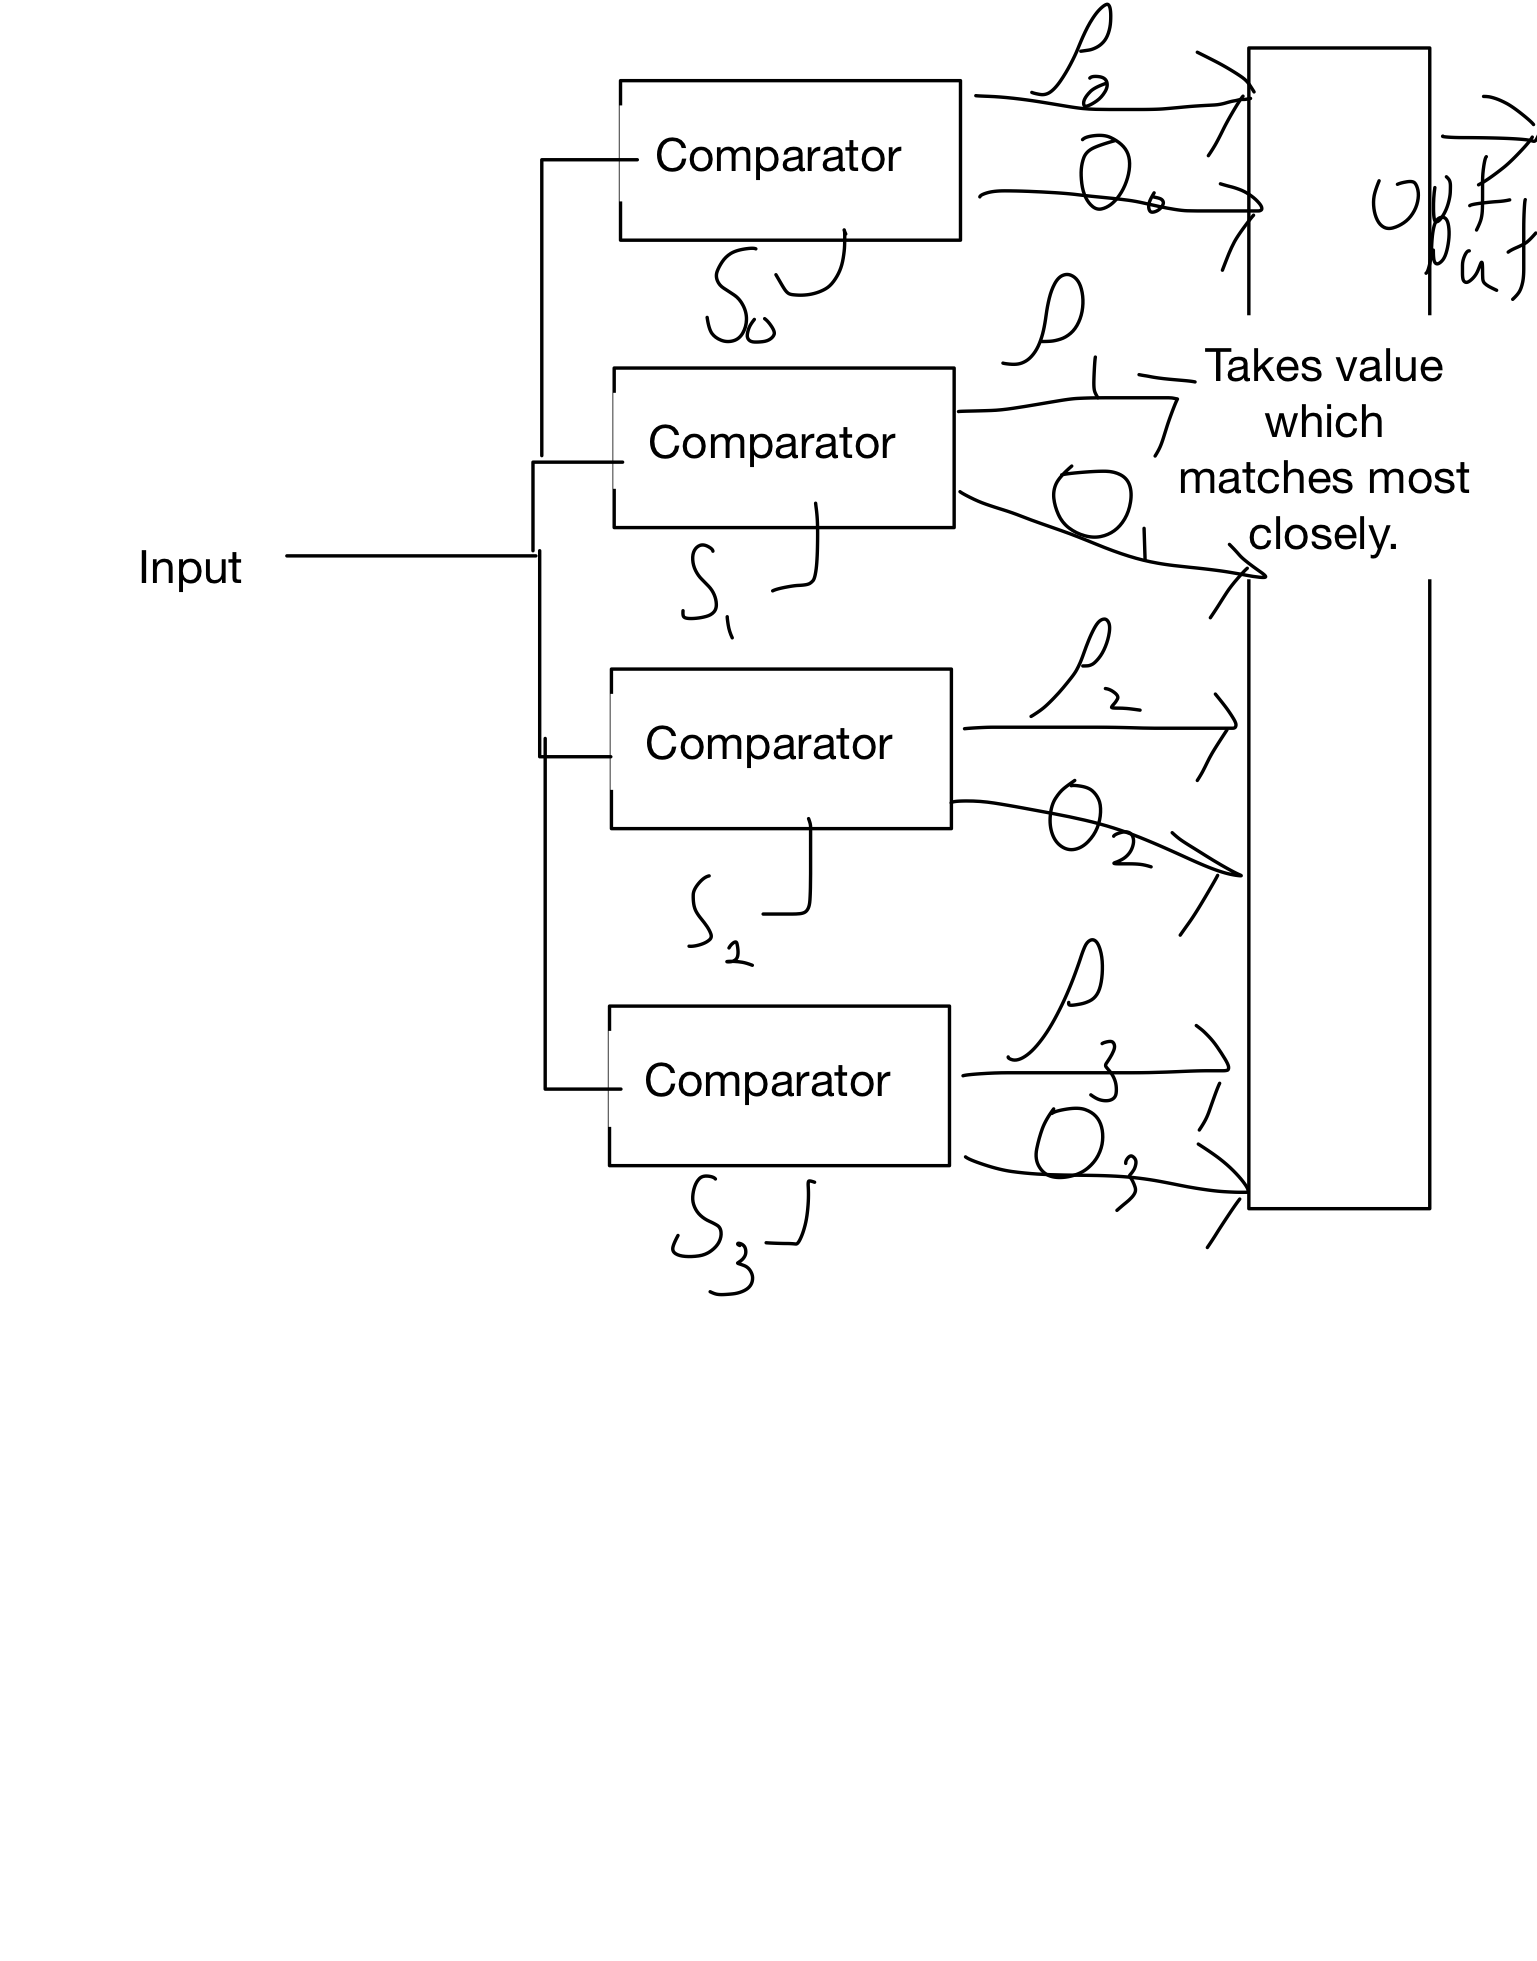
\includegraphics[width=.9\linewidth]{./img/Digital_reciever.png}
\caption{internals of Ditigal reciever with two-bit decode}
\end{figure}

\subsection{Reciever}
\label{sec-5-2}


two bits per symbol - four possible wave forms
\begin{center}
\begin{tabular}{rrl}
symbol & bits & four possible waveforms\\
0 & 00 & 0$^{\text{0}}$\\
1 & 01 & 90$^{\text{0}}$\\
2 & 10 & 180$^{\text{0}}$\\
3 & 11 & 270$^{\text{0}}$\\
\end{tabular}
\end{center}

\subsection{{\bfseries\sffamily TODO} Graham-Schmidt: check matrix algebra book on this topic.}
\label{sec-5-3}
:DEADLINE: \textit{<2018-02-05 Mon>}

\begin{itemize}
\item Signals S$_{\text{1}}$(t),\ldots{},S$_{\text{m}}$(t)
\item basis functions $\phi$$_{\text{n}}$(t),\ldots{},$\phi$$_{\text{n}}$(t), N $\neq$ M
\item \(S_i(t) = \sum{n=1}{N}{S_{in} \phi_n(t)}\)
\item \textbf{S$_{\text{i}}$} = [S$_{\text{i1}}$ S$_{\text{i2}}$ \ldots{} S$_{\text{in}}$]
\end{itemize}

\subsubsection{1st signal}
\label{sec-5-3-1}

E$_{\text{s1}}$ = $||S_{1}||^2$

\$$\phi$$_{\text{1}}$ = $\frac{S_1(t)}{\sqrt{E_{s1}}}$

$S_{11} = \sqrt{E_{s1}}$

\subsubsection{2nd -- Nth signal}
\label{sec-5-3-2}
\emph{Creating a new basis function}

S$_{\text{21}}$ = <S$_{\text{2}}$(t),$\phi$$_{\text{1}}$(t)>



r$_{\text{2}}$(t) = S$_{\text{2}}$(t) - S$_{\text{21}}$ $\phi$$_{\text{1}}$(t) <-- orthogonal to $\phi$$_{\text{1}}$(t)

\texttt{If remainted r\_i(t) = 0 skip the steps below}

\begin{itemize}
\item The part of signal 2 that can't be represented by $\phi$$_{\text{1}}$(t).

E$_{\text{r2}}$ = ||r$_{\text{2}}$(t)||$^{\text{2}}$

$\phi$$_{\text{2}}$(t) = $\frac{r_2(t)}{\sqrt{E_{r2}}}$

S$_{\text{22}}$ = $\sqrt{E_{r2}}$
\item others

S$_{\text{ni}}$ = <S$_{\text{n}}$(t) , $\phi$$_{\text{i}}$(t)> for $\phi$$_{\text{i}}$(t) which are defined.

r$_{\text{i}}$(t) = S$_{\text{i}}$(t) - $\sum$\{S$_{\text{in}}$\} $\phi$$_{\text{n}}$(t)
\end{itemize}

\subsection{Fourier Transfrom}
\label{sec-5-4}

\begin{itemize}
\item \textbf{F} \{g(t)\} = G(f) = $\int_{-\inf}^{\inf} g(t) e^{-j2\pi ft}$

\item \textbf{F} $^{-1}$ \{G(f)\} = g(t) = $\int_{-\inf}^{\inf} G(f) e^{j2\pi ft}$
\end{itemize}


\subsubsection{{\bfseries\sffamily TODO} Properties: verify that \ref{EQ1} is correct}
\label{sec-5-4-1}
\begin{itemize}
\item Linearity
\begin{itemize}
\item \textbf{F} ${a_1 x_1(t) + a_2 x_2(t)}$ = a$_{\text{1}}$ \textbf{F} ${x_1(t)}$ + a$_{\text{2}}$ \textbf{F} ${x_2(t)}$
\end{itemize}
\item Time Shift
\begin{itemize}
\item \textbf{F} ${x(t - T_0)}$ = $\int_{-\inf}^{\inf} x(t-t_0) e^{-j2\pi ft}$

$\lambda$ = t-t$_{\text{0}}$

= $e^{-j2\pi f}\int_{-\inf}^{\inf}{x(\lambda +t_0)}$

= e$^{\text{-j2}\pift_{\text{0}}}$ $\int_{-\inf}^{inf} x(\lambda) e^{-2\pi f\lambda} d\lambda$ \label{EQ1} (EQ1)

= e$^{\text{-2j}\pift_{\text{0}}}$ X(f)
\end{itemize}

\item Frequency Property
\begin{itemize}
\item \textbf{F} $^{-1}{X(f-f_0)} = e^{j2\pi f_0t} \int_{-\inf}^{\inf}{x(t)}$
\end{itemize}
\end{itemize}

\section{LEcture ?}
\label{sec-6}
:DATE: \textit{<2018-02-09 Fri>}

\subsection{Distortionless System}
\label{sec-6-1}

x(t) $->$ \box $->$ y(t)

\subsubsection{Acceptable}
\label{sec-6-1-1}
\begin{itemize}
\item Amplification//
\end{itemize}
\$y(t) = K x(t)\$//

\begin{itemize}
\item Delay \\
\end{itemize}
$y(t) = x(t-t_0)$ , \$t$_{\text{0}}$: positive integer, positive required for causality\$//

\begin{itemize}
\item Overall//
\end{itemize}
$y(t) = K x(t-t_0)$

\subsection{Freq representation}
\label{sec-6-2}

$Y(f)  = K e^{-j2\pi ft_0} X(f)$
  = $H(f)X(f)$ Linear time invariant.
where $H(f) = Ke^{-j2\pi ft_0}$

$h(t) = K\delta(t-t_0)$

\subsection{Bode rep}
\label{sec-6-3}
$H(f) = Ke^{-j2\pi ft_0}$

$\abs{H(f)} = K <- constant Mag(gain)$

$\angle{H(f)} = -2\pi ft_0 <- linear, slope = -2\pi f$


\textbf{Group Delay}: $t_g(f) = \frac{-1}{2\pi} \frac{d}{df}(\angle{H(f)})$

\subsection{Filters}
\label{sec-6-4}
\begin{itemize}
\item ideal\\
\item realistic
\begin{itemize}
\item Lowpass
\item Highpass
\item Bandpass
\item Bandstop
\end{itemize}
\end{itemize}

\begin{center}
\begin{tabular}{lll}
filter type & ideal & realistic\\
lowpass & sharp rect around center & hill flat top\\
highpass &  & \\
bandpass &  & \\
bandstop &  & \\
\end{tabular}
\end{center}
\section{LEcture ? -}
\label{sec-7}
:DATE: \textit{<2018-02-12 Mon>}
\subsection{{\bfseries\sffamily TODO} Project}
\label{sec-7-1}

\subsection{Fourier Series - Fourier Transform Relationship}
\label{sec-7-2}
\subsubsection{Fourier Series}
\label{sec-7-2-1}
F.S.    $g(t) = \sum_{-\inf}^{\inf} G_n e^{jn2\i f_0t}$

F.T.        $G(g) = *F*{g(t)}$ \&= $\sum$$_{\text{-}\inf}^{\inf}$ G$_{\text{n}}$ \textbf{F} \{e$^{\text{jn2}\pi\ \text{f}_{\text{ot}}}$\}\$
$&= \sum{G_n \delta(f-f_0)}$ -inf -> inf.\\

\subsection{Energy spectral density???????????}
\label{sec-7-3}
$E_g = \int_{-\inf}^{\inf}|G(f)|^2df$

$x(t) -> h(t) -> y(t)$ \\
   $X(f) -> H(f) -> Y(f)$

$E_y = \int_{-\inf}^{\inf}|X(f)H(f)|^2 df$
$= \int_{f_0-\detla{f}}^{f_0+|delta{f}}$
\textbf{Energy Spectral Density}
$\Psi_x (f_0) = \lim_{\Delta f -> 0}\frac{1}{\Delta f}\int_{f_0-\frac{\Delta f}{2}}^{f_0+\frac{\Delta f}{2}}|X(f)|^2 df$
$=|X(f_0)|^2$

\textbf{Energy} 
$E_x = \int \Psi_x(f) df$

\textbf{Energy int bandwith *B} centered at F$_{\text{1}}$
$\int_{-f_1-\frac{*B*}{2}}^{-f_1+\frac{*B*}{2}}\Psi_x(f) df =\int_{f_1-\frac{*B*}{2}}^{f_1+\frac{*B*}{2}}\Psi_x(f) df$
\section{{\bfseries\sffamily TODO} get units for}
\label{sec-8}
let: \$g(t) = $\Pi$(\frac{t}{\Tau}
What banwidth capacity do we need to pass exactly $90%$ of this signal energy.

$E_g = \int |g(t)|^2dt = \Tau$
\$g(t) -> "Ideal LPF bandwidth B" -> y(t) 90\%E$_{\text{g}}$ = 0.9T energy
% Emacs 25.3.1 (Org mode 8.2.10)
\end{document}
